\section*{Scratch 2 Tutorial}
\hypertarget{scratch}{}
\label{scratch}
\NewsAuthor{Horst JENS}

\textbf{Horst JENS zeigt in diesem Tutorial (welches üblicherweise während einer Probestunde bei \href{http://spielend-programmieren.at}{\textit{spielend-programmieren [1]}} verwendet wird) die Neuheiten bei der grafischen Programmieroberfläche \href{http://scratch.mit.ed}{\textit{Scratch 2.0 [2]}}. Konstruiert wird ein kleines Spiel bei welchem man Abwurfwinkel und Abwurfgeschwindigkeit einstellen muss um einen Ball auf (mehrere) Fledermäuse zu schießen.}

\subsection*{Scratch}

Die erste Version der Programmieroberfläche \textit{Scratch [1]} wurde von der Abteilung \href{http://llk.media.mit.edu/}{\textit{Lifelong Kindergarten group [3]}} des \href{http://www.media.mit.edu/}{\textit{MIT Media Labs (Massachusetts Institute of Technology [4])}},  2003 entwickelt. Scratch ist bis zur Version 1.4 freie Software (GPL Lizensiert). Der Sourcecode der neueren Version (Scratch 2.0) ist laut Scratch Homepage noch nicht verfügbar, und wird vermutlich ebenfalls frei lizensiert werden. 

Scratch 2.0 läuft rein im Webbrowser, außer einer Internet Verbindung und einem modernen Webbrowser (mit installiertem Adobe Flash) ist keine Installation erforderlich. Auf der Scratch-Website wird auch eine noch experimentelle \href{http://scratch.mit.edu/scratch2download/}{\textit{Offline-Version [5]}} zum Download angeboten

In Scratch selbst können bewegbare, animierbare Grafiken -sogenannte \textbf{Sprites}- mit Skripten programmiert werden ohne einen einzigen Befehl eintippen zu müssen. Stattdessen werden Logik-Blöcke mit der Maus aneinandergefügt, ähnlich wie Puzzle-Steine. Dadurch eignet sich Scratch sehr gut für Programmieranfänger und Schulen, um z.B. kleine Spiele, Filme oder Animationen zu erstellen. 

Scratch wird mit einigen Grafiken und Soundeffekten ausgeliefert, welche löblicherweise alle \textbf{Creative-Commons (cc-by-sa)} lizensiert sind, ebenso wie das Scratch Logo. Die mit Scratch erstellten Spiele lassen sich per Knopfdruck weltweit veröffentlichen (\textit{Share}) wodurch sie ebenfalls \textbf{cc-by-sa} lizensiert sind. Durch die \textit{look inside} Funktion kann man jedes veröffentlichte Werk auf der Scratch Website klonen (\textit{Fork}) und umbauen, ähnlich wie bei \textit{erwachsenen} \textbf{Code Repositorys}.


\subsection*{Account anlegen}

Der erste Schritt um mit Scratch zu arbeiten besteht darin sich auf der Scratch Homepage [1] (kostenlos) zu registrieren und einen Scratch Account anzulegen. Sodann kann mittels \textit{Create} Link der Scratch Programmiereditor aufgerufen werden. Man sieht das Scratch Maskottchen, eine orange Katze. Es empfiehlt sich zu diesem Zeitpunkt das Scratch Projekt zu benennen (anstatt \textit{Untitled} im Feld oben einen eigenen Namen hineintippen, z.B. \textit{Wurfdemo}) sowie die Spracheinstellung auf Englisch umzustellen (kleines Weltkugel Icon direkt rechts vom \textit{Scratch} Schriftzug oben links). Der Grund dafür ist dass in fast allen Programmiersprachen englische Befehlsnamen verwendet werden und man sich (und seinen Schülern) nichts gutes damit tut \textit{Wenn sonst} anstatt das international gebräuchliche \textit{If - Else} lernen zu lassen. Die Spracheinstellungen lassen sich jederzeit ändern.

\begin{center}
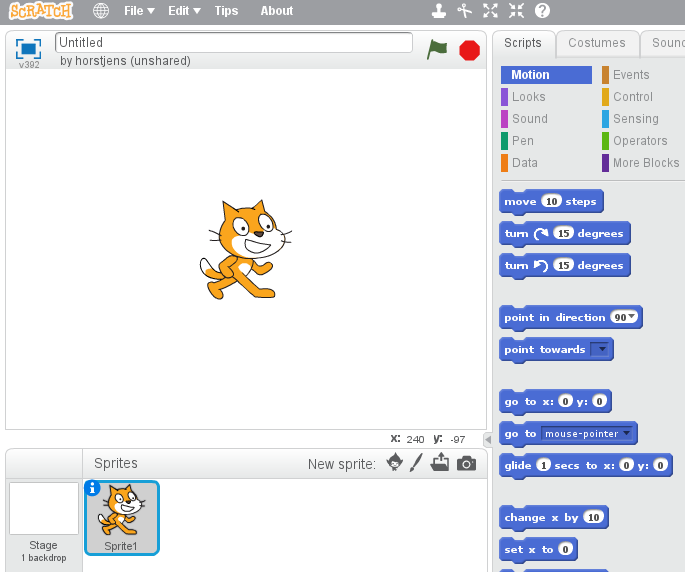
\includegraphics[width=\linewidth]{scratch/fstart.png}
\end{center}

\subsection*{Vier Sprites}

Die orange Katze kann man gleich löschen und erstellt stattdessen vier eigene Sprites: Eine Fledermaus (bat), einen Pfeil (nach rechts schauend) ein Wurfgeschoss (Basketball) sowie einen dicken grünen Strich (Wiese). Die ersten drei Sprites habe ich mit Hilfe des kleinen \textit{New Sprite} Icons aus dem Scratch Katalog übernommen, die Wiese hab ich mit Hilfe des Scratch Editors selbst gezeichnet (Vektormodus). Im Prinzip kann man alle Sprites selber zeichnen oder eigene Grafiken uploaden: Zu Beachten ist dabei dass man die Rechte an den Grafiken haben sollte (sonst gibt es legale Probleme sobald man das Scratch Spiel veröffentlicht) und dass das Wurfgeschoss absichtlich rund gewählt wurde: Bei einem runden Flugobjekt (Ball, Kanonenkugel) fällt es weniger auf wenn sich das Flugobjet nicht in Flugrichtung dreht.

\begin{center}
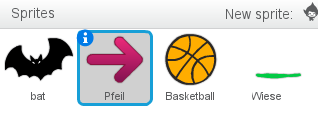
\includegraphics[width=\linewidth]{scratch/fsprites.png}
\end{center}

Noch sind alle 4 Sprites starr und unbewegt, ihnen fehlen Anweisungen (Script). Zuerst kümmern wir uns um ein paar globale Variablen:

\subsection*{Globale Variablen}

\begin{wrapfigure}{l}{3.0cm}
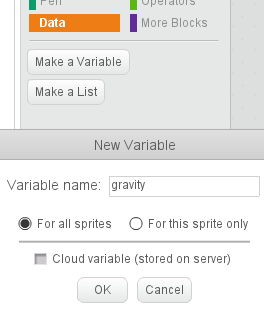
\includegraphics[width=3cm]{scratch/makevar.png}
\end{wrapfigure}
%\begin{center}
%\end{center}
Eine Variable kann man sich wie eine Sparbüchse vorstellen: Ein Behälter mit einem Namen (z.B. Klassenkassa) in dem ein sich über die Zeit ändernder Betrag drin ist. Globale Variablen bedeuten bei Scratch dass alle Sprites diese Variablen sehen (und verändern) dürfen. Für dieses Beispiel werden folgende globale Variablen benötigt: Gravitation (gravity), Winkel, Kraft, Punkte und Level. Die Namen der Variablen sind beliebig wählbar. Allerdings sollte das Zielpublikum bedenken: Wenn man mit seinem Scratch-Projekt weltweit herzeigen (share) will sind englische Namen (oder noch besser: selbst-erklärende Grafiken) besser geeignet als deutsche Namen. Man erzeugt eine Variable durch klick auf den orangen \textbf{data} Knopf in der Bildschirmmitte und danach durch Klick auf die weiße 'Make a Variable' Schaltfäche.


\begin{wrapfigure}{l}{3.0cm}
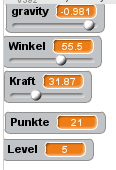
\includegraphics[width=3cm]{scratch/fsliders.png}
\end{wrapfigure}
%\begin{center}
%\end{center}
Bei Erzeugung einer globalen Variable muss der schwarze Optionskreis \textit{for all Sprites} gesetzt sein. Hat man die vier Variablen erzeugt so sieht man sie angezeigt als
orange, verschiebbare Beschriftung im Spielfeld links. Ob eine Variable überhaupt angezeigt wird kann mit einem Häkchen in der Bildschirmmitte beim Variablennamen festlegen. Die ersten drei Variablen sollen per Maus einstellbare Werte haben (Sliders): Dazu auf mit der rechten (!) Maustaste auf die Variablen-Beschriftungen klicken und erst \textit{Slider} und dann \textit{Set Slider min and max} anklicken (wie gewohnt mit der linken Maustaste). Bei Gravity habe ich -20.00 bis 0.00 gewählt (die 2 Nullen hinter dem \textbf{Dezimalpunkt} sind wichtig!), für Winkel Werte zwischen 0.00 und 90.00 und für Kraft Werte zwischen 0.00 und 100.00 - Punkte und Level bekommen keine Slider sondern dienen rein zur Anzeige der Variablenwerte.



\subsection*{Wiese}

Nun zu den Scripts für die einzelnen Sprites: Am unkompliziertesten ist das Wiesen-Sprite: Es tut gar nichts und lieft einfach nur herum. Sein Daseinszweck besteht -neben hübsch ausschauen- darin den Basketball bei Berührung erkennen zu lassen dass sein Flug vorbei ist. Mit dem Vergrößer / Verkleiner Icon (oben rechts) 

\begin{center}

\includegraphics[width=\linewidth]{scratch/fschrumpfer.png}
\end{center}

kann die Größe eines Sprites verändert werden. Die Wiese sollte den ganzen unteren Bildschirmrand ausfüllen. Wie jedes Sprite kann sie per \textit{Drag and Drop} (linke Maustaste gedrückt halten) verschoben werden.

\subsection*{Pfeil}

Relativ einfach zu programmieren ist das Skript für den (nach rechts schauenden) Pfeil. Er symbolisiert Abwurfwinkel und Abwurfgeschwindigkeit. Diese beiden \textit{globale Variablen} lassen sich sowohl per Maus als auch per Tastatur (Pfeiltasten) verändern, wenn man folgendes Skript richtig nachbaut: Das Pfeilsprite anklicken und danach folgende Befehle zusammenklicken (siehe auch vergrößerte Abbildung \textbf{Pfeilcode} am Ende dieses Artikels):

\begin{center}
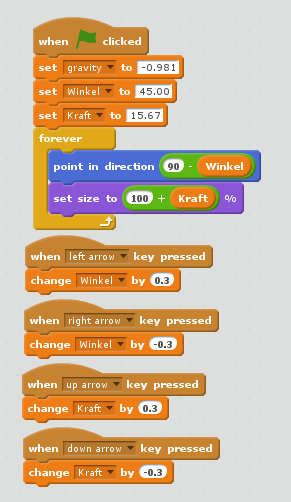
\includegraphics[width=\linewidth]{scratch/fpfeilcode.png}
\footnotesize{pfeilcode}
\end{center}

Erklärung: Falls Sie dieses Tutorial auf einem Schwarzweissdrucker ausgedruckt haben überlegen Sie sich einen Farbausdruck oder werfen Sie einen Blick auf die (bunte) online Version dieses Artikels. Die braunen, halbrunden 'Buckel' finden Sie unter dem Menüpunkt \textit{Events}. Die orangen \textit{set} (setze) und \textit{change} (verändere) Befehle finden Sie unter \textit{data}. Die gelbe \textit{forever} Schleife findet man unter \textit{Control}, den blauen \textit{point in direction} Befehl unter \textit{Motion} und den violeten \textit{set size} Befehl unter \textit{Looks}. Die grünen Minus und Plus Operatoren findet man unter -erraten- \textit{Operators}. Auch wenn man nicht versteht was die Befehle im Einzelnen tun kann man sie (sogar ohne Lesekenntnisse) nachbasteln. 

Hier die Erklärung: Die grüne Fahne (rechts oben im Spielfeld) startet das Spiel. Danach werden mit den 'set' Befehlen die Startwerte für die globale Variablen gesetzt - der letzte Spieler hat sie möglicherweise hoffnungslos verstellt. Die wie ein Schraubstock aussehende \textit{forever} Schleife wiederholt (loop) endlos die von ihr eingezwickten Befehle: Das Pfeil-Sprite dreht sich in Richtung des angegebenen Winkels (Die Berechnung (90 - Winkel) ist erforderlich da Scratch2 den Winkel 0 nach oben zeigen lässt und nicht nach rechts. Per Klick auf das blaue \textbf{i} Symbol beim Pfeilsprite kann folgende Detail-Ansicht geöffnet werden: 

\begin{center}
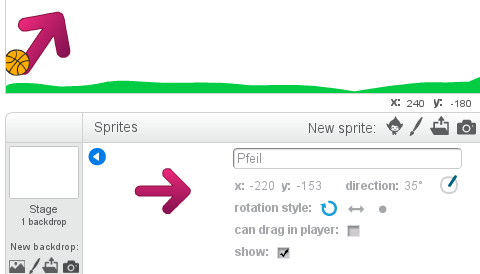
\includegraphics[width=\linewidth]{scratch/farrow.png}
\end{center}

Dort den \textit{Rotation style} auf 360 Grad (linkes Icon) einstellen.

Der \textit{set size to (100 + Kraft)\%} Befehl sorgt dafür dass der Pfeil schrumpft und wächst. Das 100+ ist notwendig damit der Pfeil auch bei einem Kraftwert von 0 sichtbar bleibt.

Die vier \textit{when key pressed} Befehle erlauben die Veränderung von Winkel und Kraft mit den Pfeiltasten.
\newpage
\subsection*{Fledermaus}
\begin{wrapfigure}{l}{3.0cm}
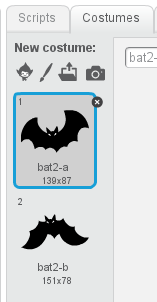
\includegraphics[width=3cm]{scratch/animation.png}
\end{wrapfigure}
Ein ganz anderes Biest ist das Skript der Fledermaus, hier ist mehr zu tun. Das Fledermaus Sprite besteht aus 2 (oder mehr) Bildern um im Spiel animiert flattern zu können. Auf das Fledermaus Sprite klicken, oben mitte auf \textit{Costumes} klicken und per Katalog-Icon (links neben dem Pinsel) ein zweites Fledermaus-Kostüm hinzufügen. Praktischerweise sind im Scratch-Katalog gleich zwei passende Fledermaus-Kostüme enthalten. Wer künstlerisch begabt ist kann noch mehr Fledermaus-Kostüme hinzufügen, dadurch schaut die Animation im fertigen Spiel flüssiger aus. Ein beliebter Trick ist es ein Kostüm öfter zu duplizieren (per Rechtsklick) und dann in jedem Kostüm z.B. die Augenfarbe zu ändern - dadurch ensteht später ein \textit{glühender Augen} Effekt der gut ausschaut und nicht allzu viel Arbeit erfordert. 

\begin{wrapfigure}{l}{3.0cm}
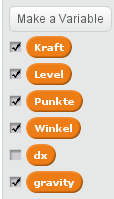
\includegraphics[width=3cm]{scratch/fbatvars.png}
\end{wrapfigure}
Zuerst einmal braucht die Fledermaus eine \textbf{private Variable}: Das Fledermaus-Sprite anklicken, von \textit{Costumes} wieder auf \textit{Scripts} wechseln,  auf \textit{Data} klicken, \textit{Make a Variable} anklicken, \textit{for this sprite only} einstellen und den Namen \textit{dx} vergeben. Diese Variable muss \textbf{nicht} ständig sichtbar sein, deshalb das Häkchen wegnehmen:

Wie man sieht bleiben die \textbf{globalen Variablen} sichtbar wenn man das Fledermaus Sprite anklickt. Die \textit{private Variable} \textbf{dx} wird unsichtbar wenn man zwischendurch ein anderes Sprite (z.B. die Wiese) anklickt. Das bedeutet das jedes Sprite unabhängig voneinander eine private Variable namens \textit{dx} haben kann, ohne dass dieses Variablen sich gegenseitig in die Quere kommen. Dx steht übrigens für delta-x und meint die Geschwindigkeit auf der X-Achse (rechts-links Bewegung). Man kann Variablen  jeden beliebigen anderen Namen vergeben.

Das Batcode-Skript ist etwas aufwendiger zu programmieren (siehe auch vergrößerte Abbildung \textbf{Batcode} am Ende dieses Artikels):

\begin{center}
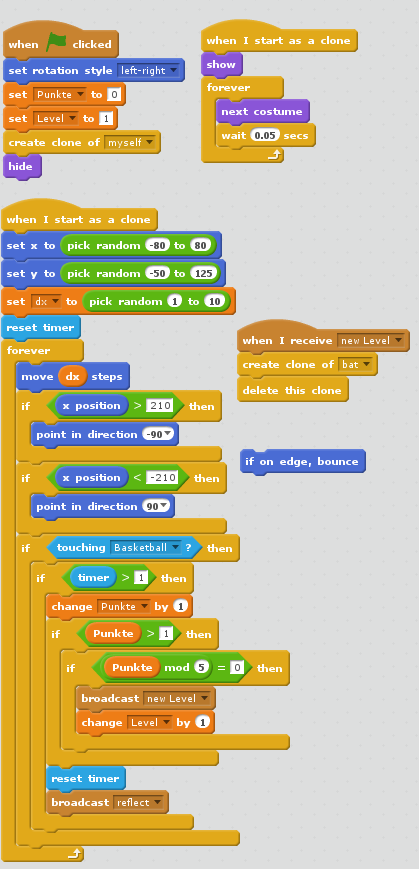
\includegraphics[width=\linewidth]{scratch/fbatcode.png}
\footnotesize{Abbildung Batcode}
\end{center}

Den blauen \textit{if on edge, bounce} Befehl habe ich nur als Erklärung dazugetan, er kann auch weggelassen werden. Da er nicht an einen 'Buckel' angedockt ist wird er sowieso nicht ausgeführt. Zur Erklärung: Der Code unter der grünen Fahne setzt zu Spielstart die globalen Variablen \textit{Level} und \textit{Punkte} auf den Wert Null macht das Fledermaus-Sprite unsichtbar. Kurz zuvor wird aber noch ein sichtbarer \textit{Klon} des Fledermaus-Sprites erzeugt. 

Der eigentliche Progammcode beginnt mit \textit{When i start as a clone}. Was macht der frisch erzeugte Fledermaus-Klon ? Er bekommt von den grünen \textit{pick random number} Befehlen eine zufällige Position (X und Y Koordinate, blau) zugewiesen und eine zufällige Geschwindigkeit (private Variable dx, orange). Danach wird per \textit{reset timer} (hellblau) eine interne Stoppuhr auf Null gesetzt und eine sehr große \textit{Forever}-Schleife abgearbeitet: Zuerst bewegt sich die Fledermaus mit der Geschwindigkeit \textit{dx} in Flugrichtung (\textit{move} Befehl, blau). Der blaue \textit{set rotation style to left-right} Befehl bei Spielstart hat dafür gesorgt dass die Fledermaus nicht nach einer Richtungsänderung mit dem Kopf nach unten fliegt. Die zwei gelben \textit{if} Befehle testen ob sich die blaue \textit{x-Position} der Fledermaus in \textit{verbotenen Bereichen} (größer als 210 oder kleiner als -210) befindet und dreht ggf. die Fledermaus in eine andere Richtung. Diesen Teil hätte eigentlich der blaue \textit{if on edge, bounce} Befehl erledigen sollen, allerdings führte dies auf meinem Computer dazu dass die Fledermaus immer wieder in der Wand hilflos flatternd stecken blieb. Die X und Y Position eines Punktes auf dem Spielfeld erfährt man indem man den Mauszeiger dorhin bewegt und die Koordniaten rechts unten unter dem Spielfeld abliest.

Danach kommt ein vierfach verschachtelter \textit{if} Befehl bei dem sich alles um eine \textbf{collision detection} mit dem Basketball dreht:

Da auf Berührung zwischen Fledermaus und Baskeball mehrmals pro Sekunde getestet wird (pro \textbf{Frame}) kann der Basketball gar nicht so schnell von der Fledermaus abprallen (dazu später mehr) und würde pro Treffer mehrere \textbf{collision detecteions} auslösen. Deshalb wird mit der Abfrage der hellblauen \textit{Timer} Variable geschaut ob seit der letzten Berührung mehr als eine Sekunde vergangen ist und erst dann weitergemacht:

In diesem Fall wird die globale Variable \textit{Punkte} um eins erhöht (change) und falls die Punktezahl glatt durch 5 teilbar ist (Punkte modulo 5 = 0) dann kommt der Spieler in den nächsthöheren Level. Dabei wird aber nicht einfach nur die globale Variable \textit{Level} erhöht sondern ein sogenannter \textbf{Event} generiert und per \textit{broadcast} Kommando verkündet. Anschließend wird die Stoppuhr per \textit{reset timer} (hellblau) wieder auf zurückgesetzt und noch ein \textit{reflect} Event per \textit{broadcast} versendet, damit der Basketball weiß dass er von der Fledermaus abprallen soll.

Parallel dazu wird ein zweiter \textit{when i start as a clone} Befehl ausgeführt: Der sorgt dafür dass die Fledermaus sichtbar ist (\textit{show}, violett) und wechselt alle 0.05 Sekunden (\textbf{Dezimalpunkt!}) das Fledermaus-Kostüm - dadurch entsteht der Flatter-Effekt oder die Animation.

Am seltsamsten ist vermutlich der braune \textit{When i receive next Level} Befehl: Hier wird erst ein neuer Fledermaus-Klon generiert und danach der aktuelle Klon gelöscht mit \textit{delete this clon}. Warum ? Ich empfehle einfach den \textit{delete this clon} Befehl einmal wegzulassen und das fertige Spiel ein paar Runden zu spielen: Exponentielles Fledermauswachstum droht ! Meine Erklärung: Jede Fledermaus, auch die unsichtbare 'Ursprungs' Fledermaus, reageiert auf den \textit{NextLevel-Event}. Wenn eine unsichtbare und eine sichtbare Fledermaus jeweils einen sichtbaren Klon erzeugen gibt es bei Level 2 ( 2 x 2 = 4 - 1 = 3) schon drei  Fledermäuse. Bei Level 3 (4 x 2 = 8 - 1 = 7) sind es dann schon sieben sichtbare Fledermäuse, bei Level 4 schon ( 8 x 2 = 16 - 1 = 15) fünfzehn usw. 

\subsection*{Basketball}

Nun zum schwierigsten Sprite-Skript, dem für den Basketball. Zunächst braucht der Baksetball gleich drei unsichtbare  \textit{private Variablen}, nämlich \textit{dx, dy} und \textit{fliegt}. Letztere ist ein sogenanntes \textit{Flag} oder auch \textit{boolsche Variable}: Sie soll nur zwei verschiedene Werte annehmen können, nämlich: \textit{Der Basketball fliegt} oder eben  \textit{Der Basketball fliegt nicht}. In Scratch wird das durch die beiden Werte Eins (fliegt) und Null (fliegt nicht) realisiert. 

\begin{wrapfigure}{l}{2.0cm}
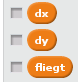
\includegraphics[width=2cm]{scratch/fballvars.png}
\end{wrapfigure}
Delta-X und Delta-Y hingegen sind \textit{Vektoren}\footnote{Der Mathematiklehrer Ihres Vertrauens äußert sich sicher gerne ausführlichst zu diesem Thema} und geben die Fluggeschwindigkeit in der X-Achse (links-rechts) bzw in der Y-Achse (oben-unten) an. Beide zusammengenommen beschreiben ob der Ball \textit{schräg} fliegt. 

Würde man noch eine Varibale für Delta-Z sowie eine für die Z-Position erzeugen dann ließe sich mit Scratch ein perspektivisches 3D Spiel realisieren - Ein Beispiel für den \textbf{B.E.} Unterricht finden Sie auf \href{http://spielend-programmieren.at/en:tutorials:centralperspective}{\textit{verlinkt auf meiner Homepage [6]}}

Der Code für den Ball benutzt die dunkel-violette \textit{More Blocks} Funktionalität von Scratch2 um ein Subprogramm zu realisieren 
(siehe auch vergrößerte Abbildung \textbf{Ballcode} am Ende dieses Artikels):
\begin{center}
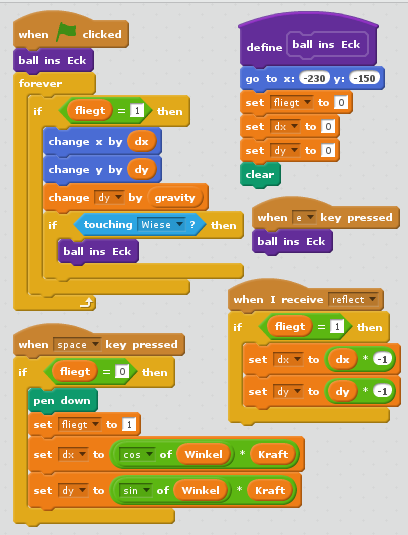
\includegraphics[width=\linewidth]{scratch/fballcode.png}
\footnotesize{Abbildung Ballcode}
\end{center}

Die \textit{Ball ins Eck} Subroutine wird von drei verschiedenen Stellen aufgerufen und stellt den Ball wieder in die Ecke links unten, knapp über die Wiese.

\textit{Delta-X} und \textit{Delta-Y} werden über die Cosinus- bzw. Sinus-Funktion von Scratch berechnet: dorthin fliegt der Ball. Die Schwerkraft (gravity) zieht die ganze Zeit über den Ball nach unten und verändert sein Delta-Y. Wenn der Basketball die Wiese berührt oder die Taste e gedrückt wurde hört er auf zu fliegen und wird in die Ecke teleportiert. Außerdem lauscht der Basketball auf den \textit{reflect} Event welcher von einem beliebigen Fledermaus-Klon ge\textit{broadcastet} werden kann: In diesem Fall drehen sich Delta-X und Delta-Y um, der Ball wird reflektiert. 

Geschickte Spieler können den Ball zwischen mehreren Fledermäusen reflektieren lassen. 

Der grüne \textit{Pendown} Befehl sorgt dafür dass der Ball eine (treppenförmige) Flugbahn zeichnet, der grüne \textit{clear} Befehl löscht diese Spur wieder weg. Beide Befehle befinden sich im grünen \textit{Pen} Menü.

\begin{center}
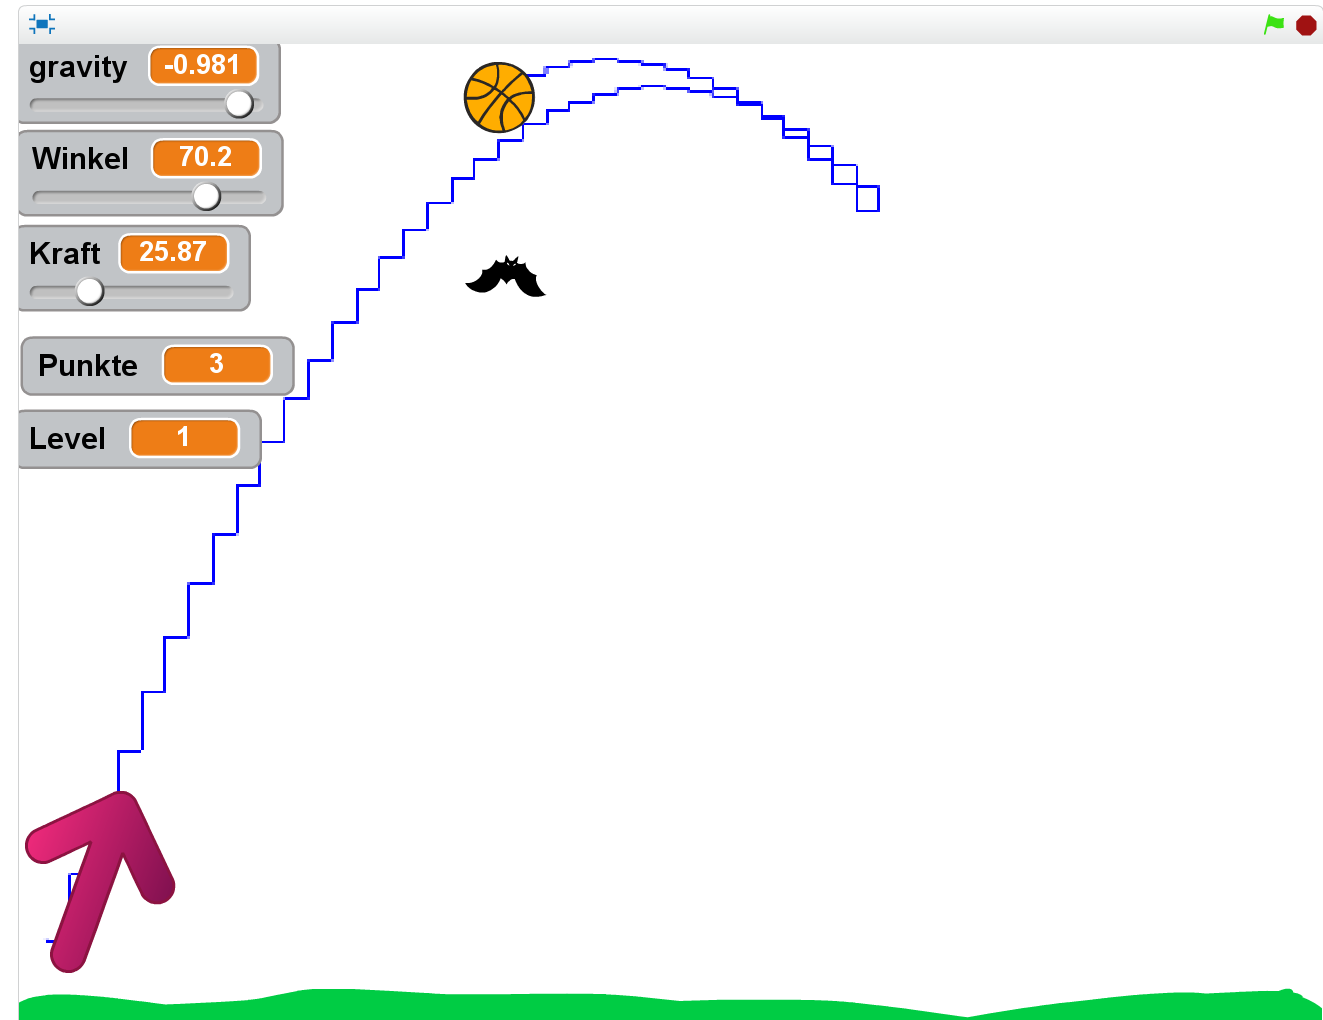
\includegraphics[width=\linewidth]{scratch/final.png}
\footnotesize{Fledermaus wurde im Flug getroffen reflektiert den Basketball}
\end{center}


\subsection*{Fachbegriffe}

~~~~\href{https://de.wikipedia.org/wiki/Sprite_(Computergrafik)}{\textbf{Sprite}} (englisch: Geist) bewegbare Computergrafik, z.B. der Mauszeiger.\\

\href{https://en.wikipedia.org/wiki/Source_code_repository}{\textbf{Code Repository}} eine Website auf der (Open Source) Code-Projekte gesammelt und verwaltet werden um weltweites gemeinsames Arbeiten zu ermöglichen. Beispiel. \href{http://github.com}{\textit{github.com}}\\

\textbf{Collision Detection}: Kollisionserkennung, üblicherweise zwischen zwei Sprites oder zwischen einem Sprite und einer Hintergrundfarbe. \\

\textbf{Frame, Framerate, Frames per Second (fps)} gibt an wie viele Einzelbilder (Frames) der Comptuer pro Sekunde (FPS) anzeigt um die Illusion einer Bewegung zu erzeugen. Ein idealer Wert sind 60 \textit{frames per second}, der aber speziell von schwächeren Computern und komplexen Spielen mit vielen Sprites nicht erreicht wird. Unter 10 FPS wird ein Spiel unangenehm ruckelig. \\

\textbf{Event} englisch: Ereignis. Bei Scratch berichtet ein Skript per \textit{broadcast} (=herumschreien, funken) allen anderen Sprites von einem Ereignis. Diese können per \textit{when i recive broadcast} darauf reagieren. \\


\subsection*{Lizenz, Quellen:}
\begin{wrapfigure}{l}{2.0cm}

\includegraphics[width=2cm]{powdertoytutorial/ccbysa88x31.png}
\end{wrapfigure}
Dieses Material steht unter der Creative-Commons-Lizenz Namensnennung - Weitergabe unter gleichen Bedingungen 4.0 International. Um eine Kopie dieser Lizenz zu sehen, besuchen Sie \url{http://creativecommons.org/licenses/by-sa/4.0/deed.de}.

\subsection*{Download, Feedback:}
\textbf{R.I.S.-Journal}, Ausgabe 001: \\
\href{http://spielend-programmieren.at/de:ris:001}{spielend-programmieren.at/de:ris:001}\\
\textbf{Download} Ordner, verschiedene Formate: \href{http://spielend-programmieren.at/risjournal/001/scratch}{\texttt{spielend-programmieren.at/\\risjournal/001/scratch}} \\
\textbf{Feedback} \Letter\ \texttt{horst.jens@spielend-\\programmieren.at} \\


\textbf{Quellen:} \\
{[}1{]} \href{http://spielend-programmieren.at}{spielend-programmieren.at}\\
{[}2{]} \href{http://scratch.mit.edu}{Scratch.mit.edu}\\
{[}3{]} \href{http://llk.media.mit.edu/}{llk.media.mit.edu}\\
{[}4{]} \href{http://www.media.mit.edu/}{www.media.mit.edu}\\
{[}5{]} \href{http://scratch.mit.edu/scratch2download/}{scratch.mit.edu/scratch2download}\\
{[}6{]} \href{http://spielend-programmieren.at/en:tutorials:centralperspective}{goo.gl/ClnYs0} \\

%\SepRule
%\begin{multicols}{2}
\end{multicols} % !!!!!!!!!!!!!!!!!!!!!!!!
\begin{center}
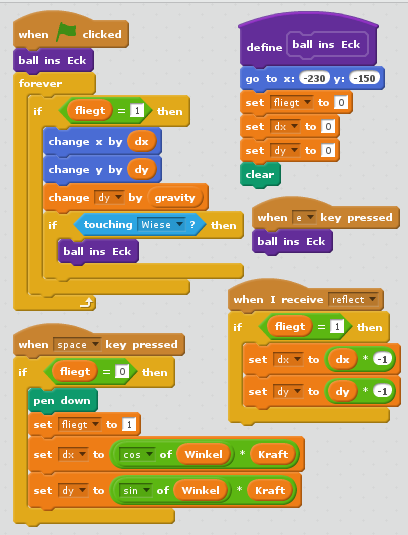
\includegraphics[width=0.7\linewidth]{scratch/fballcode.png}\\
\footnotesize{Ballcode}
\end{center}

\begin{minipage}{0.35\linewidth}  
\begin{center}
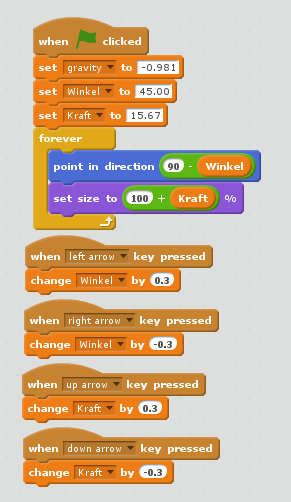
\includegraphics[width=\linewidth]{scratch/fpfeilcode.png}
%\footnotesize{Pfeilcode (lin}
Abbildungen: Pfeilcode (links), Batcode (rechts)
\end{center}
\end{minipage}
\begin{minipage}{0.6\linewidth}
\begin{center}
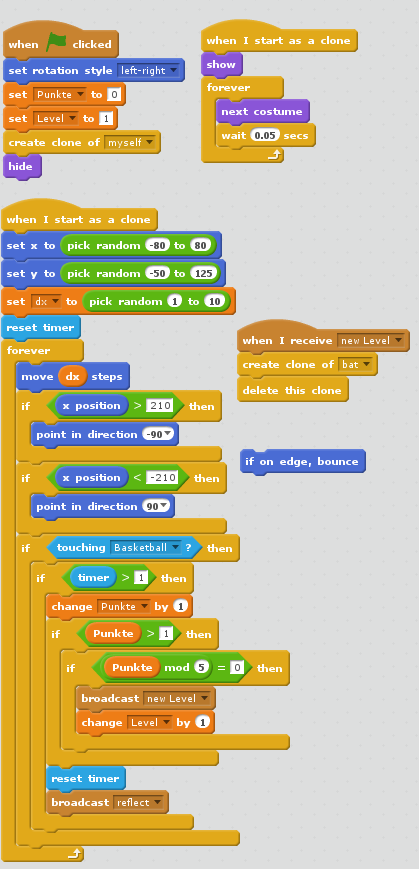
\includegraphics[width=\linewidth]{scratch/fbatcode.png}
%\footnotesize{Batcode}
\end{center}    
\end{minipage}
